\subsection{Rate-limited, repetition 1}
\begin{figure}[H]\centering
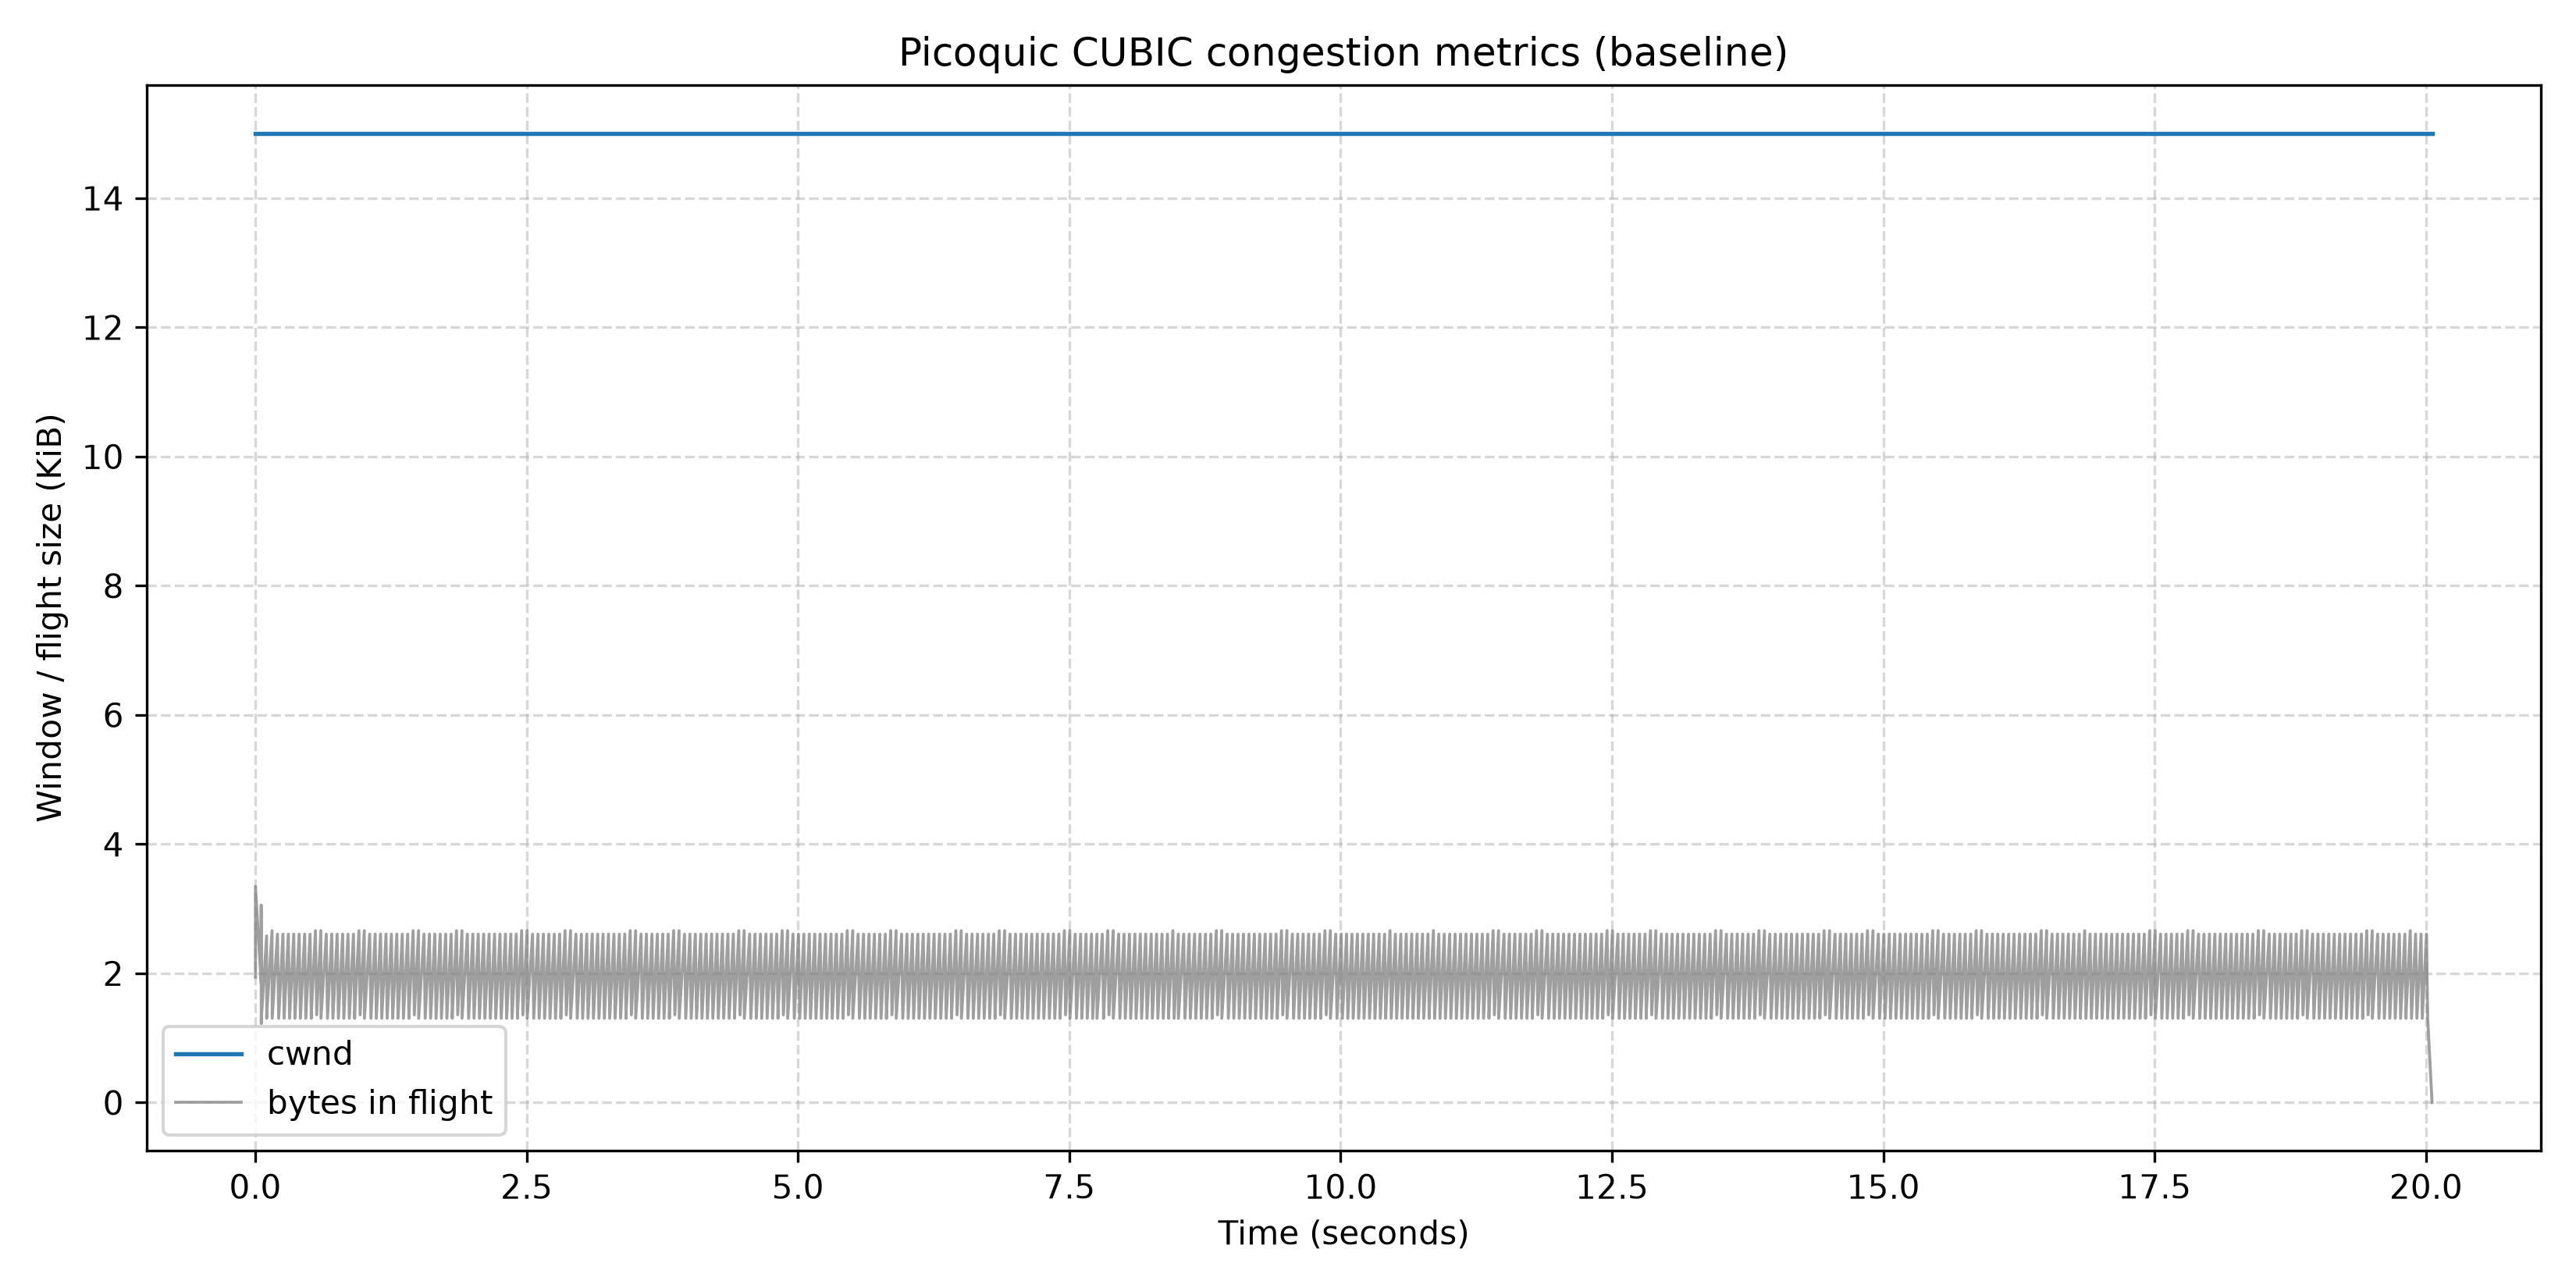
\includegraphics[width=0.92\textwidth]{plots/rate-limited-baseline-1.png}
\caption{Baseline: final cwnd 15.00 KiB; time-weighted mean 15.00 KiB; throughput 0.190 Mbit/s.}\end{figure}
\begin{figure}[H]\centering
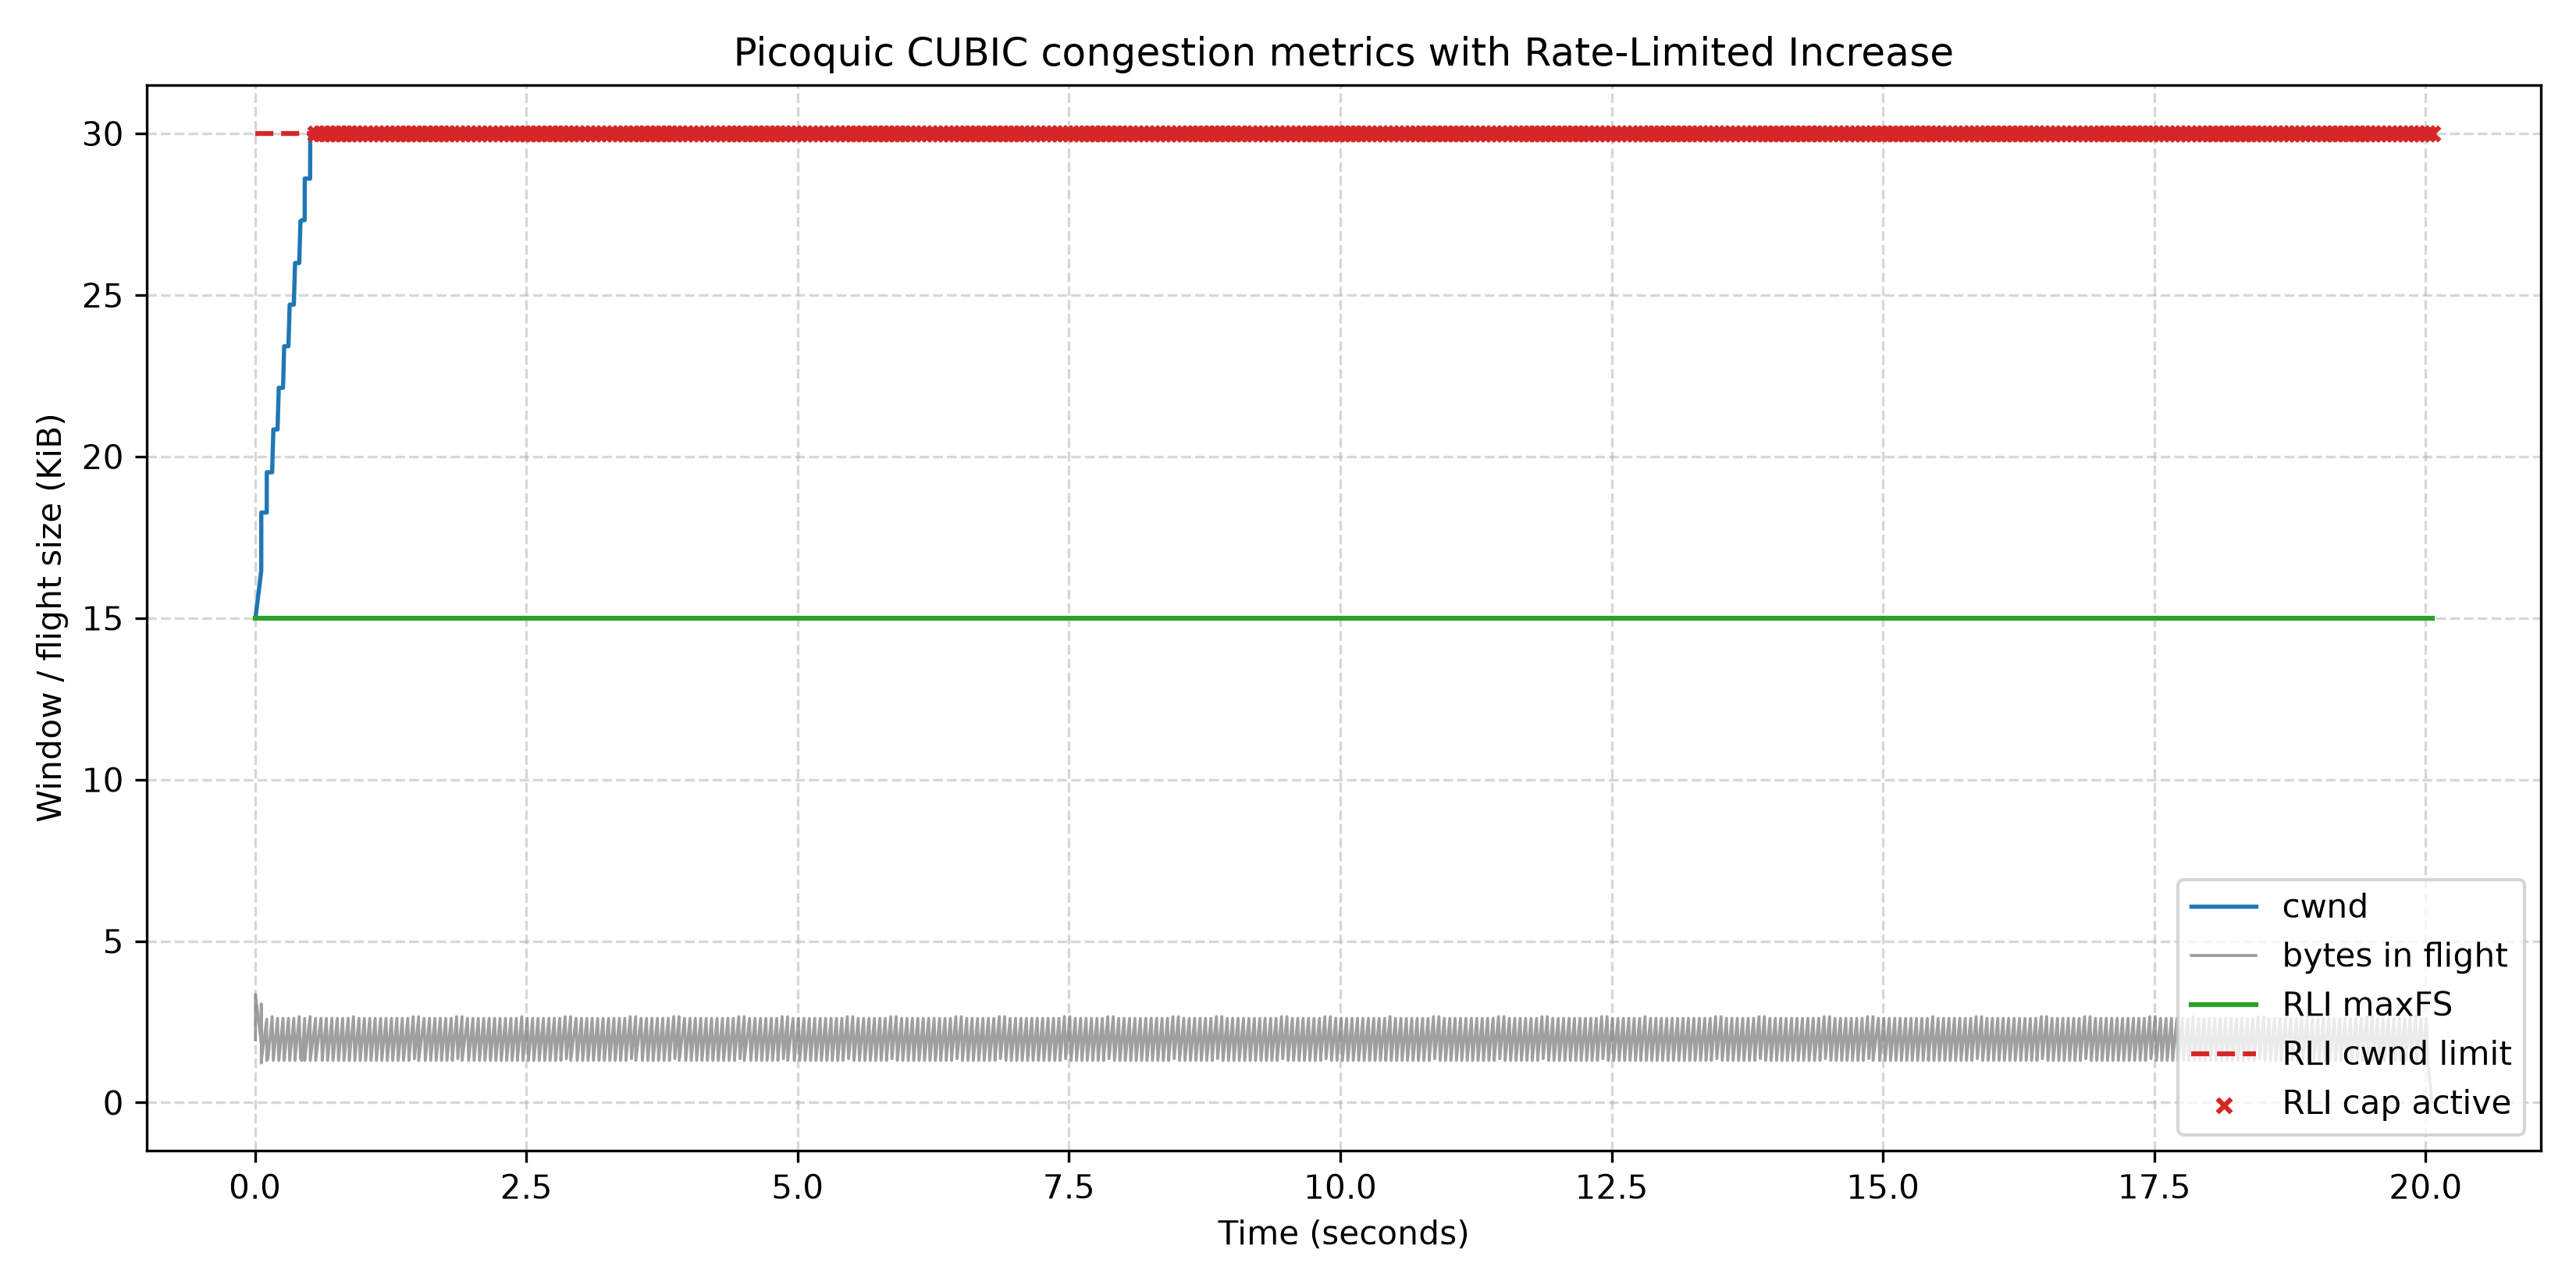
\includegraphics[width=0.92\textwidth]{plots/rate-limited-rli-1.png}
\caption{RLI: final cwnd 30.00 KiB; time-weighted mean 29.81 KiB; throughput 0.190 Mbit/s.}\end{figure}
RLI allows window growth up to its cap. The application supplies the same limited data in both runs.
\clearpage\subsection{Bulk control, repetition 1}
\begin{figure}[H]\centering
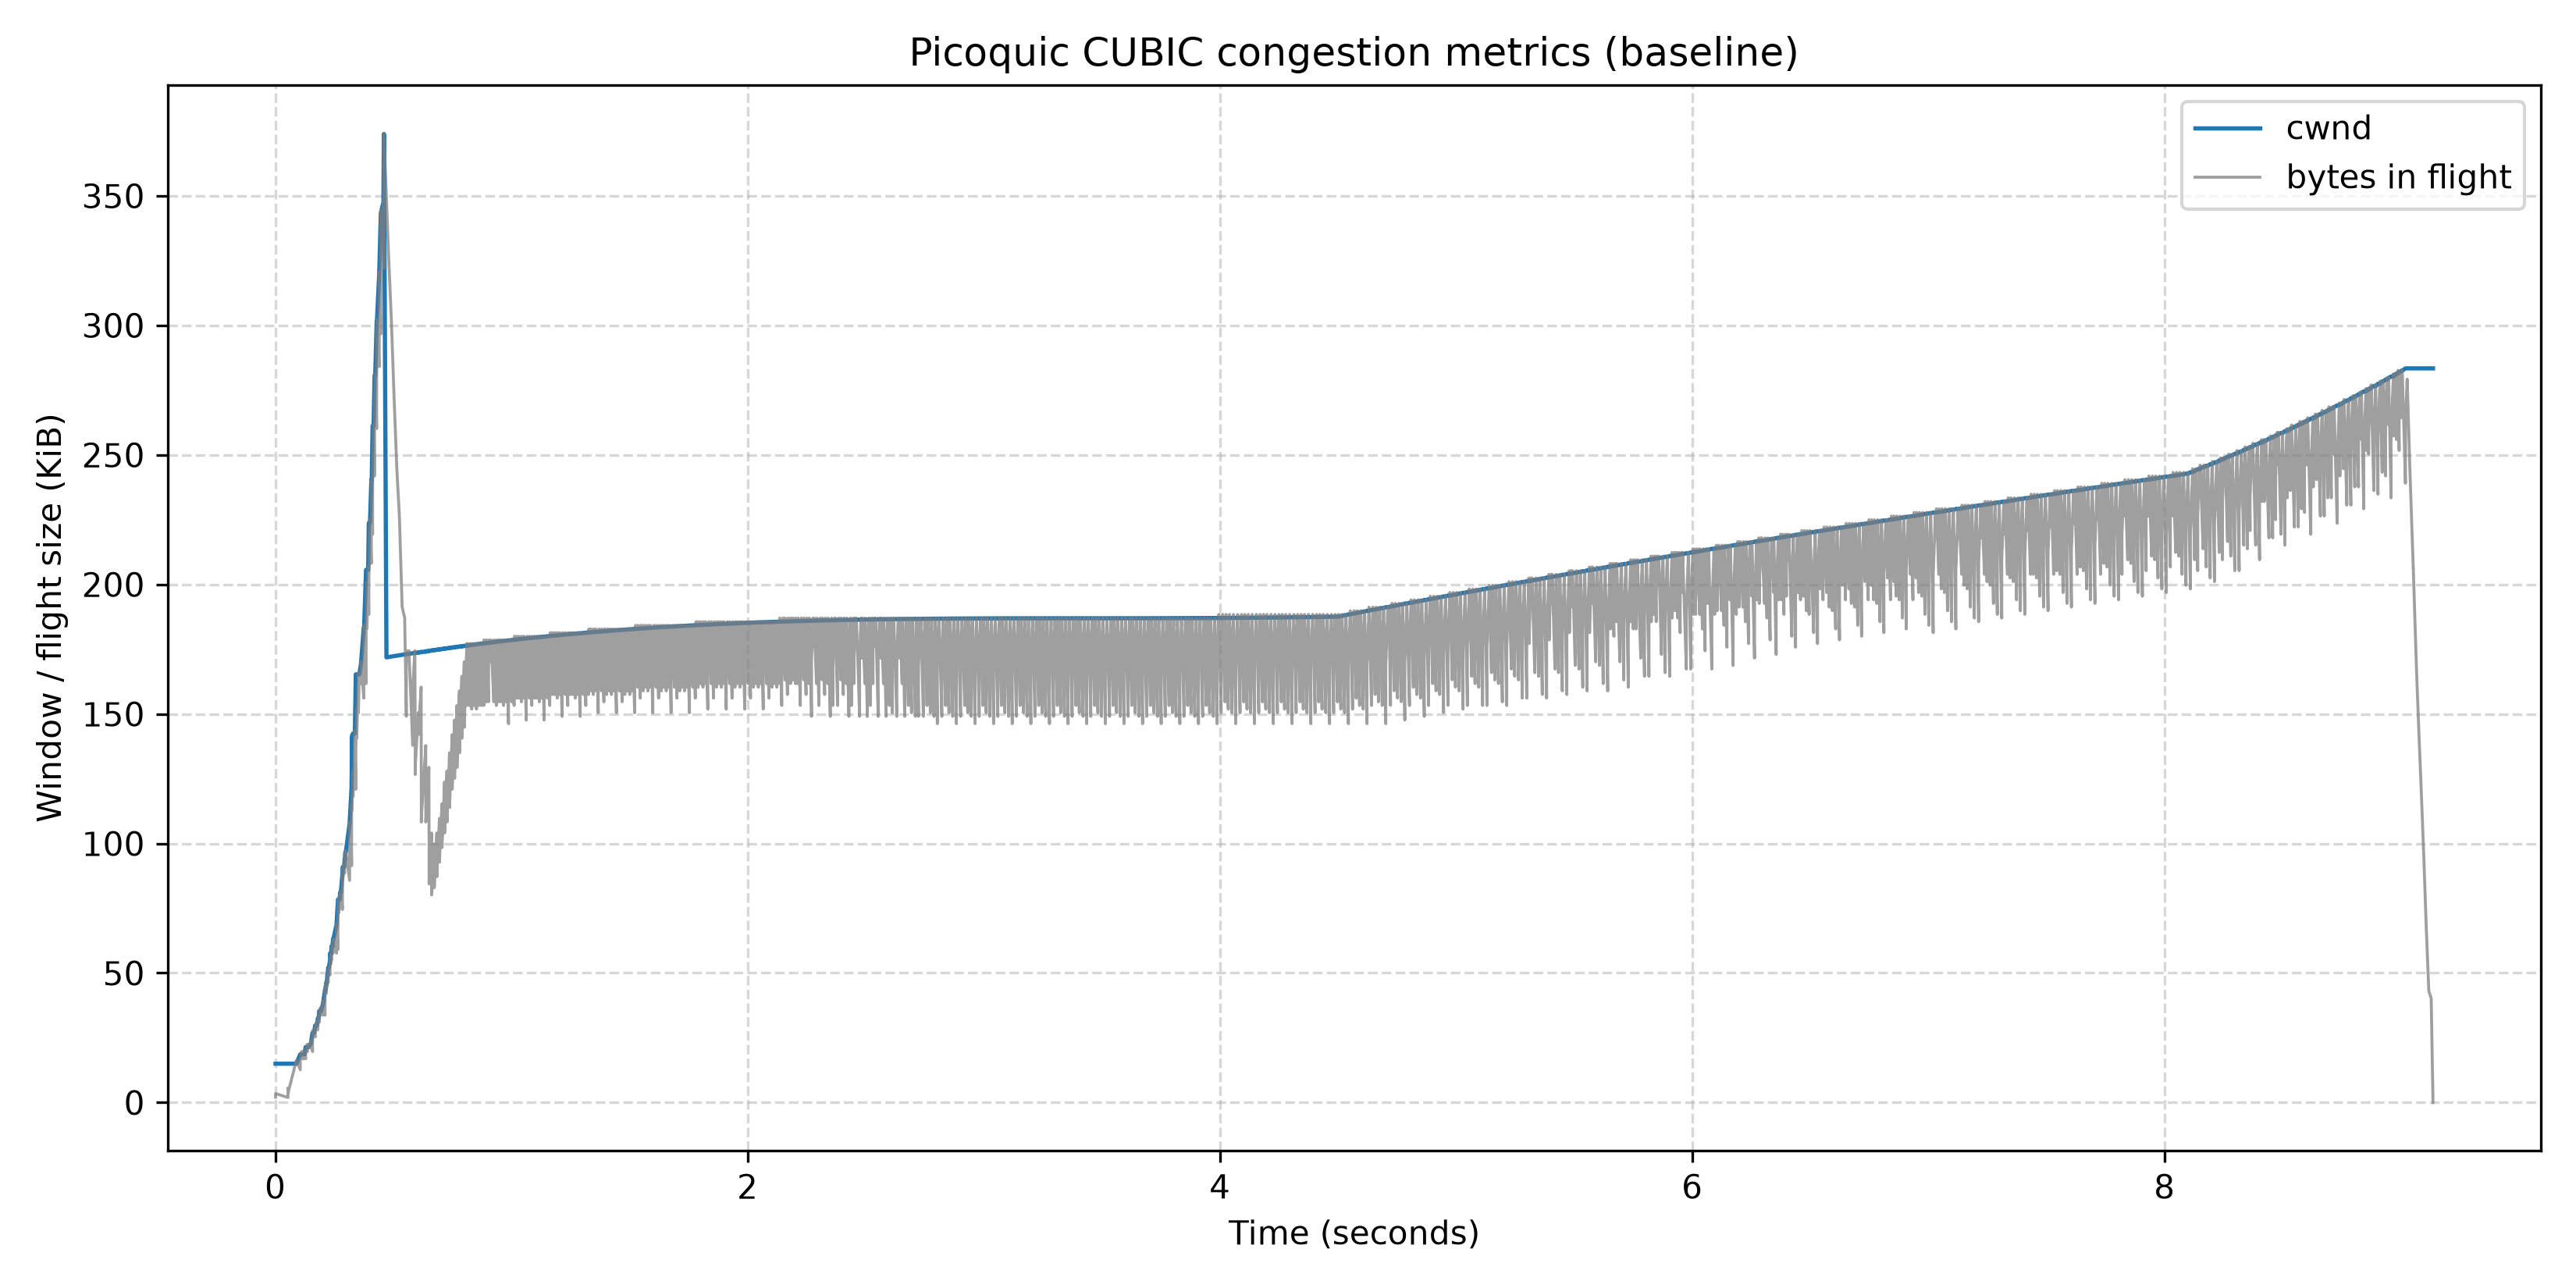
\includegraphics[width=0.92\textwidth]{plots/bulk-baseline-1.png}
\caption{Baseline: final cwnd 283.41 KiB; time-weighted mean 201.63 KiB; throughput 17.731 Mbit/s.}\end{figure}
\begin{figure}[H]\centering
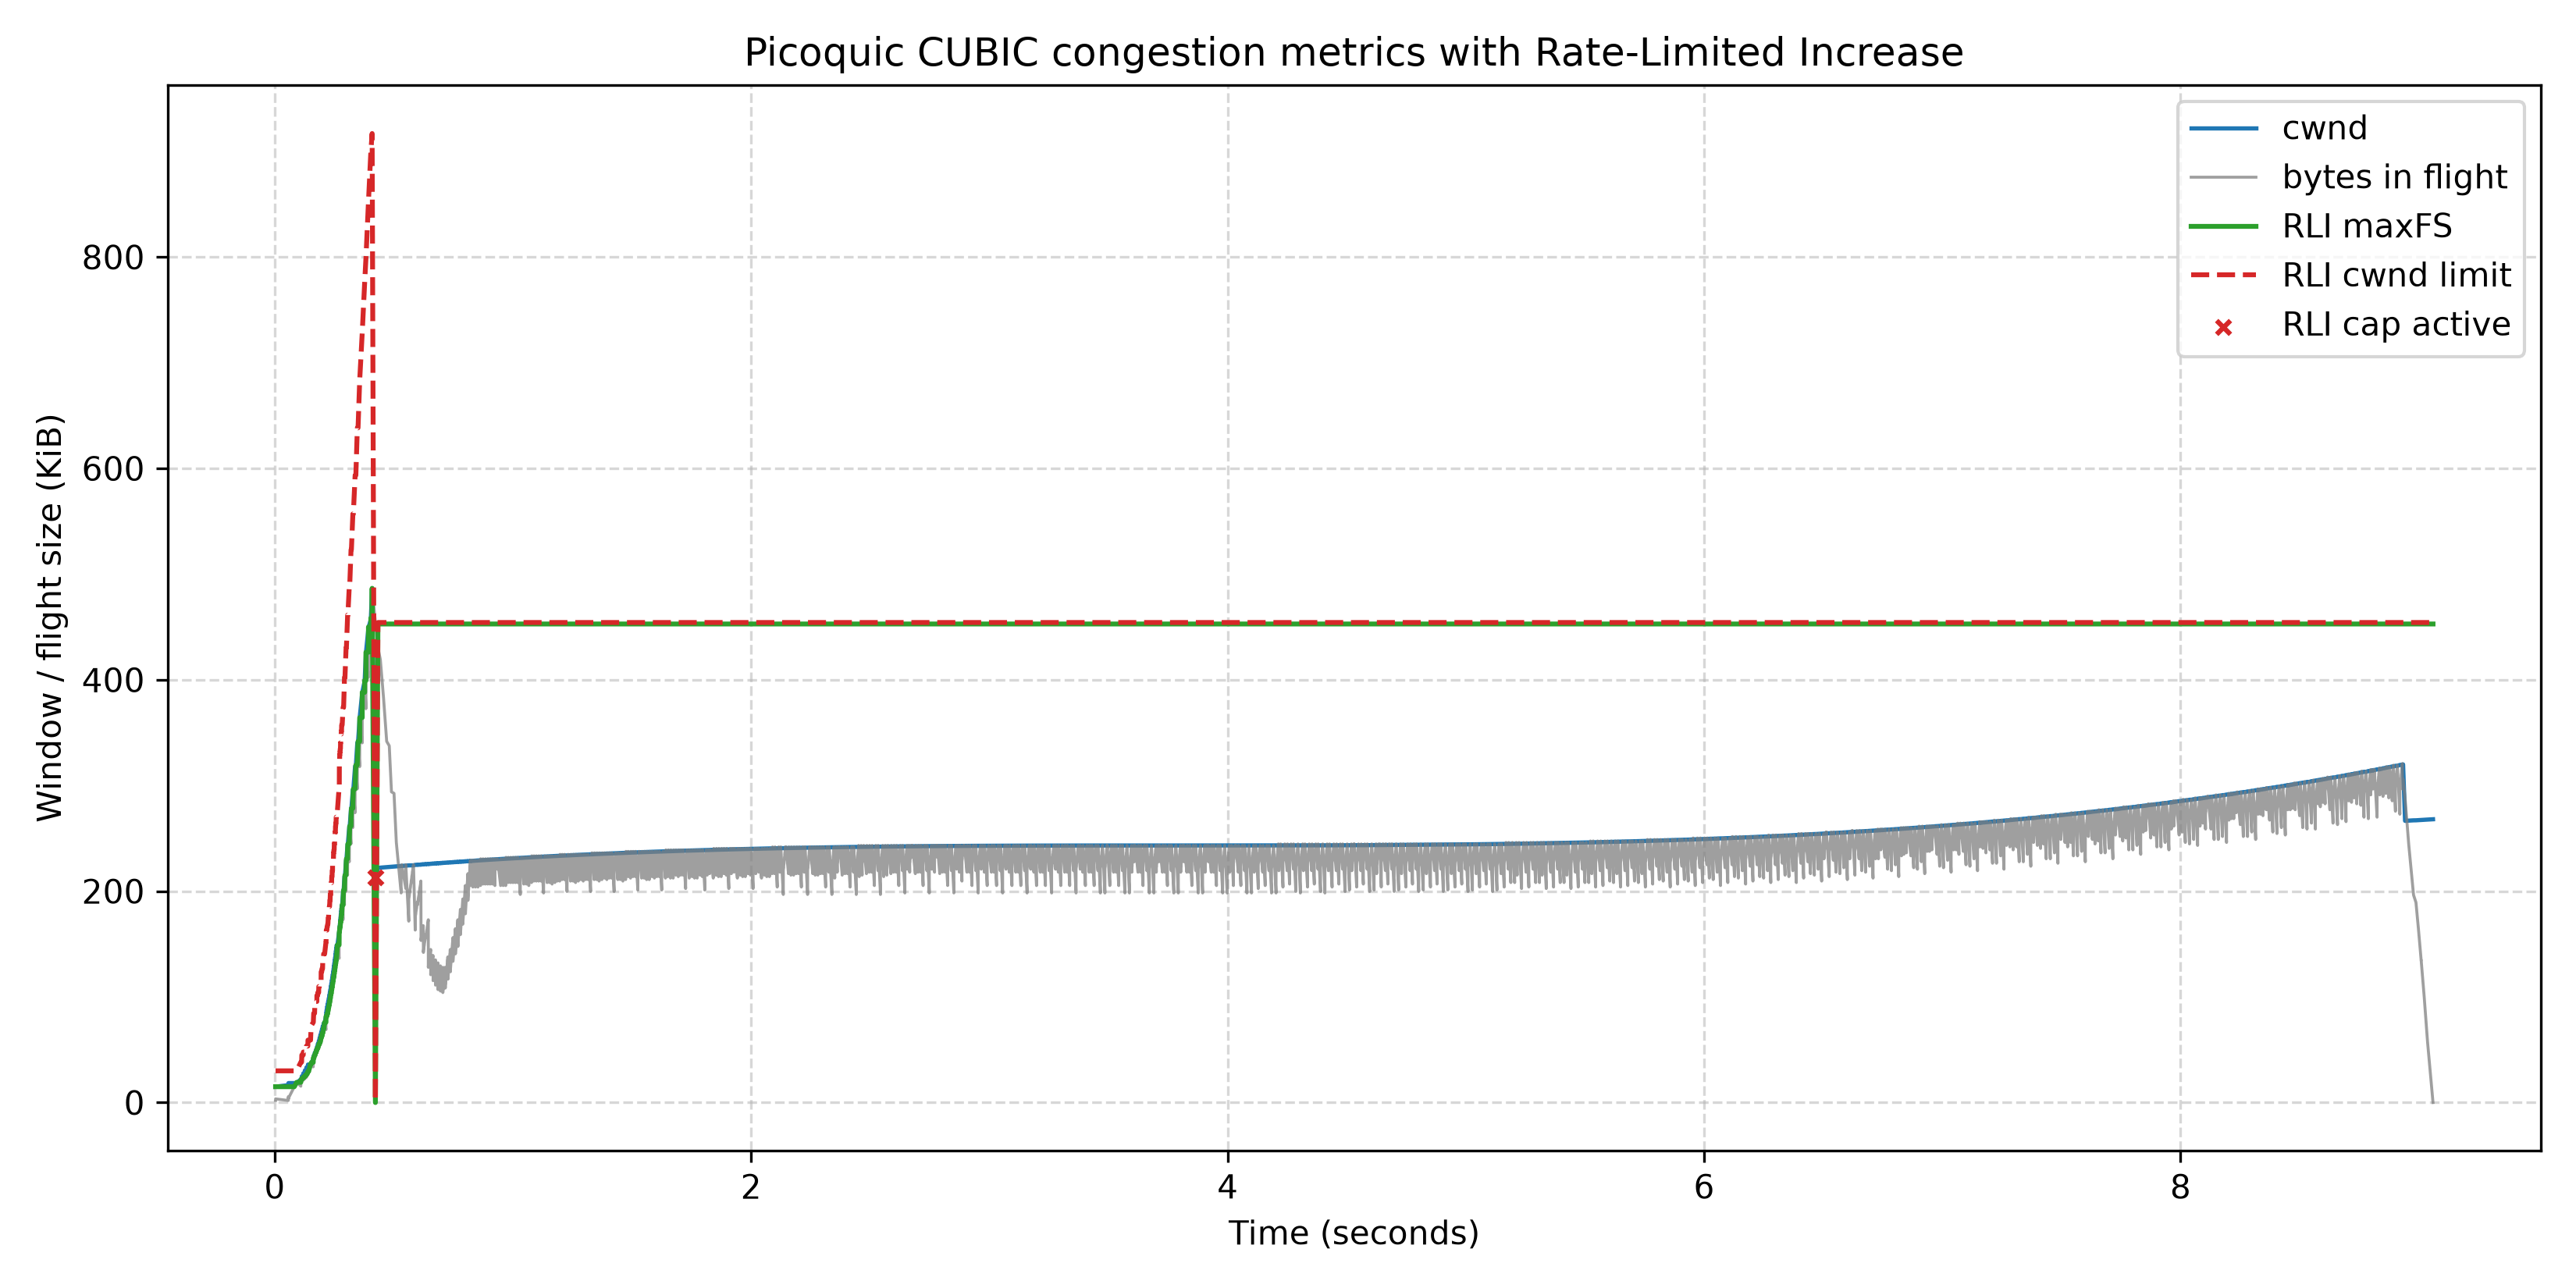
\includegraphics[width=0.92\textwidth]{plots/bulk-rli-1.png}
\caption{RLI: final cwnd 268.04 KiB; time-weighted mean 248.21 KiB; throughput 17.940 Mbit/s.}\end{figure}
Both senders have continuous data. Use the measured throughput to compare the runs; cwnd height alone does not show transfer speed.
